\chapter{Demostración práctica}
Para complementar el trabajo teórico, se incluye un archivo Jupyter Notebook con
implementaciones de juguete de ideas y algoritmos vistos. Además, se utiliza el
conocimiento adquirido en el trabajo anterior (\textit{Dashboards}) para generar
datos de prueba y visualizarlos de manera interactiva utilizando \textit{Voila}.

\section{Distancia de Mahalanobis con distribuciones multivariantes}
Para esta demostración, se genera una distribución multivariante usando \\
\Verb#numpy.random.multivariate_normal# y haciendo que el umbral que define si un dato
es anómalo o no sea interactivo.

\noindent
\begin{minipage}{\linewidth}
	\centering
	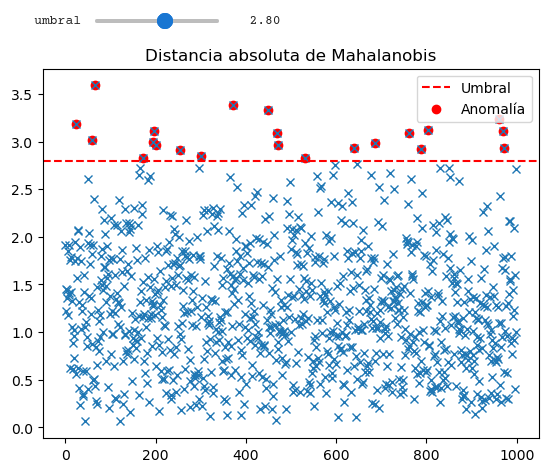
\includegraphics[width=\textwidth]{demo/mahalanobis_abs.png}
	\captionof{figure}{Plot de las muestras por distancia absoluta de Mahalanobis}\label{fig:demo11}
\end{minipage}

\noindent
\begin{minipage}{\linewidth}
	\centering
	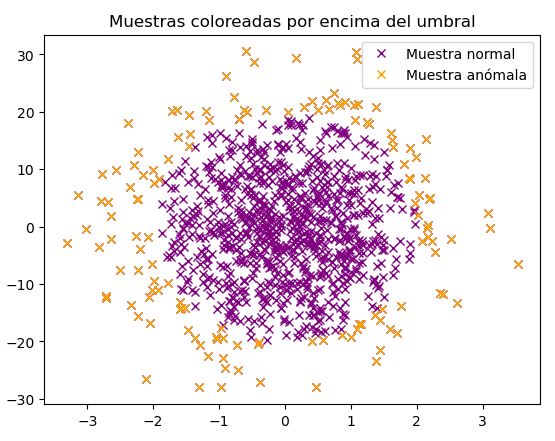
\includegraphics[width=\textwidth]{demo/mahalanobis_space.png}
	\captionof{figure}{Conjunto coloreado por anomalías}\label{fig:demo12}
\end{minipage}

\section{Detección de anomalías basada en proximidad}

\section{Detección de anomalías basada en clusters}

\section{Preprocesado de datos y minería de excepciones en sistema KLNX}
